%%%%%%%%%%%%%%%%%%%%%%%%%%%%%%%%%%%%%%%%%%%%%%%%%%%%%%%%%%%%%%%%%%
%%%%%%%% ICML 2017 EXAMPLE LATEX SUBMISSION FILE %%%%%%%%%%%%%%%%%
%%%%%%%%%%%%%%%%%%%%%%%%%%%%%%%%%%%%%%%%%%%%%%%%%%%%%%%%%%%%%%%%%%

% Use the following line _only_ if you're still using LaTeX 2.09.
%\documentstyle[icml2018,epsf,natbib]{article}
% If you rely on Latex2e packages, like most moden people use this:
\documentclass{article}

% For figures
\usepackage{graphicx} % more modern
%\usepackage{epsfig} % less modern
\usepackage{subfigure} 
\usepackage{natbib}
\usepackage{amssymb}
\usepackage{amsmath}
\usepackage{amsfonts}
\usepackage{amsthm}
\usepackage{mathtools}
%\usepackage{algorithm2e}
% For algorithms
\usepackage{algorithm}
\usepackage{algorithmic}

% As of 2011, we use the hyperref package to produce hyperlinks in the
% resulting PDF.  If this breaks your system, please commend out the
% following usepackage line and replace \usepackage{icml2013} with
% \usepackage[nohyperref]{icml2013} above.
\usepackage{hyperref}

% Packages hyperref and algorithmic misbehave sometimes.  We can fix
% this with the following command.
\newcommand{\theHalgorithm}{\arabic{algorithm}}

% Employ the following version of the ``usepackage'' statement for
% submitting the draft version of the paper for review.  This will set
% the note in the first column to ``Under review.  Do not distribute.''

\usepackage{icml2013} 
% Employ this version of the ``usepackage'' statement after the paper has
% been accepted, when creating the final version.  This will set the
% note in the first column to ``Proceedings of the...''
% \usepackage[accepted]{icml2013}
\newtheorem{theorem}{Theorem}
\newtheorem{lemma}{Lemma}
\newtheorem{remark}{Remark}
\newtheorem{corollary}{Corollary}

% The \icmltitle you define below is probably too long as a header.
% Therefore, a short form for the running title is supplied here:
\icmltitlerunning{2-bits Compressive Sensing with Use Case in Radio Astronomy}

\begin{document} 
\setlength{\abovedisplayskip}{5.5pt}
\setlength{\belowdisplayskip}{6pt}

\twocolumn[
\icmltitle{2-bits Compressive Sensing with Use Case in Radio Astronomy}

% It is OKAY to include author information, even for blind
% submissions: the style file will automatically remove it for you
% unless you've provided the [accepted] option to the icml2013
% package.
\icmlauthor{Nezihe Merve G\"{u}rel}{nezihe.guerel@inf.ethz.ch}
\icmladdress{Eidgen�ssische Technische Hochschule Z�rich,
            314159 Pi St., Palo Alto, CA 94306 USA}
\icmlauthor{Your CoAuthor's Name}{email@coauthordomain.edu}
\icmladdress{Their Fantastic Institute,
            27182 Exp St., Toronto, ON M6H 2T1 CANADA}

% You may provide any keywords that you 
% find helpful for describing your paper; these are used to populate 
% the "keywords" metadata in the PDF but will not be shown in the document
\icmlkeywords{compressed sensing, low precision, iterative hard thresholding, radio astronomy, fpga}

\vskip 0.3in
]

\begin{abstract} 
Iterative Hard Thresholding (IHT) algorithm offers near optimal recovery of compressible signals sampled below the Nyquist rate. IHT, however, seems to have a computational bottleneck when applied to the compressed sensing recovery problems with general (non-Gaussian) dense measurement matrices. To relieve this, we propose to compress the measurement matrix by quantizing the bit-widths of its entries at each iteration. This low precision framework results in runtime efficiency on hardware yet still maintaining the stability and performance guarantees of the algorithm. To demonstrate this, we first derive theoretical error bounds for sparse signal recovery. Under certain constraints, low precision IHT is shown to converge with near-optimal error guarantees. We then illustrate through simulation the potential for Radio Astronomy  with achievement of 7.7x speed up on Field-Programmable Gate Array. An application to Low Frequency Array leads to a better resolution of the sky sources recovered with order of magnitude speed up. 
\end{abstract} 
\section{Introduction}
%Back through the decades, the breakthrough foundation of signal acquisition was the Nyquist-Shannon sampling theorem, namely a band-limited signal can be recovered from its samples perfectly if the sampling rate is at least twice the highest frequency component.
%The recently emerging field of compressed sensing is a foundational technique in sparse signal reconstruction. Acquiring a signal with sparse representation in some transform domain, i.e., Wave

1- CS

2- IHT-NIHT-Comparison

3- Quantization

\subsection{Paper Overview}

\subsection{Notation}
Scalars are denoted by italics, vectors by bold lower-case and matrices by bold upper-case. For all ${\bf x}= (x_1, \hdot, x_n) \in \mathbb{R}^n$, we denote by $\|{\bf x}\|_p = (\sum_{i=1}^n x_n^p)^{1/p}$ the standard ${\ell}_p$-norm and by
where $H_s({\bf x}): \mathbb{C}^n \rightarrow \mathbb{C}^n$ the nonlinear operator that preserves the largest $s$ (in magnitude) entries of {\bf x} and sets the remaining to zero. 
\section{Iterative Hard Thresholding}
In this section, we review the preliminary results on the normalized Iterative Hard Thresholding (IHT) algorithm introduced by [refs].

\subsection{Definition of the Algorithm} 
Let ${\bf x}^{[0]} = 0$, the normalized IHT$_s$ has the following update rule per iteration
\begin{equation}\label{iht_update_rule}
{\bf x}^{[n+1]} = H_s({\bf x}^{[n]} + \mu^{[n]}{\bf \Phi}({\bf y}-{\bf \Phi}{\bf x}^{[n]})),
\end{equation}
where $\mu^{[n]}>0$ is the adaptive step size parameter. %Under certain conditions, the normalized IHT converges to a local minimum of the optimization problem
%\begin{equation}\label{cost_function}
%    \textrm{min} \|{\bf y}-{\bf \Phi x} \|_2^2
%\ \ \ {\textrm{subject \ to }}\ \ \|{\bf x}\|_0 \leq s.
%\end{equation}

\subsection{Convergence} 
The analysis of the heavily relies on the scaling properties of ${\bf \Phi}$. More precisely, the converge to a local minimum of the cost function $\|{\bf y}-{\bf \Phi x} \|_2$ was proven under certain conditions on the measurement matrix: ${\bf \Phi}$ as well as the performance guarantees. To be more concrete on these conditions, one must often deal with non-symmetric Restricted Isometry Property (RIP), namely, a matrix ${\bf \Phi}$ satisfies non-symmetric RIP if
\begin{equation}\label{rip}
\alpha_{s} \leq \frac{\|{\bf \Phi} {\bf x}\|_2}{\|{\bf x}\|_2} \leq \beta_{s}
\end{equation}
for all ${\bf x}: \|{\bf x}\|_0 \leq s$, and some $\alpha_s, \beta_s \in \mathbb{R}$ such that $0<\alpha_s\leq \beta_s$. the so-called Restricted Isometric Constants (RICs).
\begin{remark}
The convergence of normalized IHT depends conditionally on the step size parameter $\mu^{[n]}$ unlike the traditional IHT approach where $\mu^{[n]}=1$. While the traditional approach merely requires a re-scaling of measurement matrix such that $\|{\bf \Phi}\|_2 <1$ to ensure convergence, introducing a step size parameter to compensate for this re-scaling avoids undesirable amplification of noise, i.e., the ratio of $\|{\bf \Phi x}\|_2/\|{\bf e}\|_2$ remains unchanged. 
\end{remark}

The main convergence result an be stated as follows. Proof can be found in, for example, [ref].

\begin{theorem}
{\rm{\cite{niht}}}\\ 
Let ${\bf \Phi}$ is of full rank and $s\leq m$. If $\beta_{2s}\leq\mu^{-1}$, then normalized IHT converges to a local minimum of ref{costfunc}.
\end{theorem}

\subsection{Step Size Determination} 
While setting the step size parameter, the condition that $\beta_{2s}\leq\mu^{-1}$ ensuring convergence poses the following challenge. To date, there is no universal strategy known to check if the RIP holds for an arbitrary measurement matrix in a computationally efficient manner. Similar discussion holds for attaining the RICs, i.e., ${\beta_s}$ and $\alpha_s$, associated with the measurement matrix ${\bf \Phi}$. It could however be shown that, under certain conditions, ran-
domly constructed measurement matrices can satisfy
the RIP with high probability []. Still, it remains a bottleneck for a more general class of
measurement matrices. Without losing the main track, here we intend to review a more generic strategy for step size determination.

If the support is fixed, a natural strategy to set the step size adaptively is []
\begin{equation}\label{step_size}
   \mu^{[n]} = \frac{{\bf g}^T_{\Gamma^{[n]}}{\bf g}_{\Gamma^{[n]}}}{{\bf g}^T_{\Gamma^{[n]}}{\bf \Phi}^T_{\Gamma^{[n]}}{\bf \Phi}_{\Gamma^{[n]}}{\bf g}_{\Gamma^{[n]}}}
\end{equation}
where ${\bf g}^{[n]} = {\bf \Phi}^T({\bf y}-{\bf \Phi x}^{[n]})$. Clearly, the maximal reduction in cost function can then be attained. However, if the support of ${\bf x}^{[n+1]}$ differs than that of ${\bf x}^{[n]}$, the sufficient condition to guarantee convergence is [ref44ofgreedy]
\begin{equation}
    \mu^{[n]} \leq(1-c) \frac{\|{\bf x}^{[n+1]}-{\bf x}^{[n]} \|_2^2}{\|{\bf \Phi}({\bf x}^{[n+1]}-{\bf x}^{[n]}) \|_2^2},
\end{equation}
for any small constant $c$.

If the above condition is not met, a new proposal for ${\bf x}^{[n+1]}$ can be calculated by using $\mu^{[n]}\leftarrow{\mu^{[n]}/(k(1-c))}$, where $k$ is a shrinkage parameter such that $k>1/(1-c)$.

This adaptive setting of step size parameter is shown to provide RIP-invariant convergence result by [ref] as follows.
\begin{theorem}
{\rm{\cite{niht}}}\\
If rank({${\bf \Phi}$}) = m and rank(${\bf \Phi}$_{\Gamma}) = s \ $\forall \Gamma:\ |\Gamma| = s$, then the so-called normalized IHT algorithm converges to a local minimum of the cost function ref.
\end{theorem}
\subsection{Recovery Performance.} 
 In a series of papers [...], extensive research effors have been made and strong theoretical guarantees were derived. Here we state the most refined recovery error bounds.
\begin{theorem}
{\rm{\cite{niht}}}\\
Consider a noisy observation ${\bf y} = {\bf \Phi x} + {\bf e}$ with an arbitrary vector {\bf x}. Also, assume ${\bf \Phi}}$ is non-symmetric RIP$_{2s}$ and let $\gamma_{2s} = \beta_{2s}/\alpha_{2s}-1$. If $\gamma_{2s} \leq {1}/{8}$, then
\begin{equation}
    \| {\bf x}-{\bf x}^n\|_2 \leq 2^{-n}\| {\bf x}^s\|_2 + 8\tilde{{\bf \epsilon}_s}\label{niht_error_bound}
\end{equation} where \begin{equation}
    \tilde{{\bf \epsilon}_s} =  \| {\bf x}-{\bf x}^s\|_2 + \frac{\| {\bf x}-{\bf x}^s\|_1}{\sqrt{s}}+\frac{1}{\beta_{2s}}\|{\bf e} \|_2.
\end{equation}

Remarkably, after at most $n^*=\log_2(\|{\bf x}^s\|_2/\tilde{\bf \epsilon}_s)$ iterations, the recovery error bound in \ref{niht_error_bound} can be further simplified to
\begin{equation}
   \| {\bf x}-{\bf x}^n\|_2 \leq 9\tilde{{\bf \epsilon}_s}.
\end{equation}
\end{theorem}
The above result suggests that, after a sufficiently large number of IHT runs, the reconstruction error is induced only by the noise ${\bf e}$ and that ${\bf x}$ is not exactly s-sparse.




\section{Low Precision Iterative Thresholding}
In this section, we present the proposed accelerated Iterative Hard Thresholding and establish rigorous performance guarantee for sparse signal recovery. The key development here is that, by reducing the bit widths used to represent the dense measurement matrices as well as measurements, we still obtain near-optimal recoveries. 

Let ${\bf x}^{[0]} = 0$ and use iteration
\begin{equation} \label{modified_update_rule}
  {\bf x}^{[n+1]} = H_s\big({\bf x}^{[n]}+\mu Q_b(\boldsymbol{\Phi})(Q_b({\bf y})-Q_b(\boldsymbol{\Phi}){\bf x}^{[n]})\big)  
\end{equation}
where $Q(\cdot)$ is the quantization function that maps single-precision floating-point onto a codomain where each element has $b$-bits precision.

{\bf Quantization Scheme:} We employ a stochastic quantization function denoted with $Q_b({\bf v})$, where ${\bf v}=(v_1, v_2, .., v_d) \in \mathbb{R}^d$ is an arbitrary vector and $b$ is the total number of bits used to represent it. {\bf v} can then be quantized into $l=2^b$ levels as follows. Let $\ell_i$, $i\in \{1, 2, ..., l-1 \}$ denote $l$ equally spaced points on $[\min({\bf v}), \max({\bf v})]$ such that $\ell_1=\min({\bf v})$, $\ell_l=\max({\bf v})$ and $\ell_1\leq\ell_2 \leq ... \leq \ell_l$, also $v_j$ for $j\in \{1, 2, ..., d \}$ fall into the interval $[\ell_i, \ell_{i+1}]$. Then we assign the probabilities to the nearest levels as
\[
    Q_b(v_j) = \left\{\begin{array}{lr}
        \ell_i, & \textrm{with probability} \ \frac{\ell_{i+1}-v_j}{\ell_{i+1}-\ell_i}\\
        \ell_{i+1},&\textrm{otherwise}.  \ \ \ \  \ \ \ \ \ \ \ \ \ \ \ \ \ \ 
        \end{array}
\]
  
Remark that the above equation yields that the quantization operation $Q(\cdot)$ is unbiased, i.e., $\mathbb{E}[Q_b({\bf v})] = {\bf v}$. Also, let $\hat{{\bf v}}$ represent the quantized ${\bf v}$ and drop $Q(\cdot)$ to simplify notational burden. The detailed steps of the algorithm is then given in Algorithm \ref{low_precision_iht}.



\begin{algorithm}[h!]
   \caption{Low Precision Iterative Hard Thresholding}
   \label{low_precision_iht}
\begin{algorithmic}
   \STATE {\bfseries Input:} Measurement matrix ${\bf \Phi}$, measurements ${\bf y}$, sparsity parameter $s$, number of iterations $n^*$, $b_{\bf \Phi}$ and $b_{\bf y}$ 
   \REPEAT
   \STATE Initialize ${\bf x} = 0$, $\mu = $.
   \FOR{$i=1$ {\bfseries to} $n-1$}
   \STATE ${\bf g}^{[i]} = Q^{\dagger}_{b_{\bf \Phi}}({\bf \Phi}) \big(Q_{b_{\bf y}}({\bf y})-Q^{\dagger}_{b_{\bf \Phi}}{\bf x}^{[i]}\big)$
   \STATE ${\bf x}^{[i+1]} = H_s({\bf x}^{[i]} + \mu {\bf g}^{[i]})$
   \ENDFOR
   \UNTIL $n = n^*$
\end{algorithmic}
\end{algorithm}
{\bf Convergence:} The modified algorithm attains a local minimum of the cost function $\mathbb{E} [ \| \hat{\bf y} - \hat{\bf \Phi}{\bf x}\|_2^2]$ such that $\|{\bf x}\|_0 \leq s$. This can be majorized by the following surrogate objective function 
\begin{equation*}
    \begin{split}
        \mathbb{E} [\|\mu^{0.5}\hat{\bf y} -   \hat{\bf \Phi}{\bf x}\|_2^2+ \|{\bf x} 
    - {\bf x}^{[n]} \|_2^2
    - \|\mu^{0.5}\hat{\bf \Phi}({\bf x}- {\bf x}^{[n]}) \|_2^2] 
    \end{split}
\end{equation*}
whenever $\| \mu^{0.5}\hat{\bf \Phi}\|_2^2 <1$. If this condition is met, the minimizer of the above surrogate objective: ${\bf x}^{[n+1]}$ ensures that $\| \hat{\bf y} - \hat{\bf \Phi}{\bf x}^{[n+1]}\|_2^2 \leq \| \hat{\bf y} - \hat{\bf \Phi}{\bf x}^{[n]}\|_2^2$. Moreover, by using the arguments of [], \ref{modified_update_rule} can be shown to minimize the expected cost $\mathbb{E} [ \| \hat{\bf y} - \hat{\bf \Phi}{\bf x}\|_2^2]$.

{\bf Computational Complexity:} The iterative thresholding algorithm involves two vector additions and two dense matrix multiplication as well as thresholding operation per iteration. Low precision approach thus alleviates the computations by blabla and reduces memory requirements to store the dense measurement matrix ${\bf \Phi}$. (we need to improve here)
 
{\bf Conditions on $\hat{\Phi}$:} Unlike the traditional approach, the normalized iterative hard thresholding algorithm where $\mu$ is no longer unity enables the arbitrary scaling of measurement matrix by relaxing the bounds of the norm of $\hat{{\bf \Phi}}$. The restricted isometry property holds for the quantized measurement if
\begin{equation}
    \hat{\alpha}_{s} \leq \frac{\|\hat{{\bf \Phi}} {\bf x}\|_2}{\|{\bf x}\|_2} \leq \hat{\beta}_{s}
\end{equation}
$\forall {\bf x}: \| {\bf x}\|_0 \leq s$. The resctricted isometry constants $\hat{\alpha}_s$ and $\hat{\beta}_s$ can therefore be re-scaled accordingly with $\hat{\bf \Phi}$.

{\bf Step Size Determination:} The step size $\mu$ is required to counteract the scaling of $\hat{{\bf \Phi}}$ such that $\|\mu^{0.5} \hat{\bf\Phi}\|_2^2 <1$ to ensure the convergence. This yields the trivial bound on $\mu$ as
\begin{equation}
    1/\hat{\beta}_s^2 < \mu < 1/\hat{\alpha}_s^2.
\end{equation}
Moreover, using \ref{step_size} in the low precision setting, we can initially determine $\mu$ to guarantee the convergence without requiring the knowledge of the restricted isometry constants.

 \subsection{Performance Guarantees}
 Convergence is necessary to guarantee the existence of a stable scheme for sparse signal recovery. However, the recovery performance of such algorithms is of our primary interest. The following theorem states the recovery error by explicitly exhibiting the component introduced by the quantization.
\begin{theorem}\label{main_theorem_TH}
Given a noisy observation ${\bf y} = {\bf \Phi x}+{\bf e} $ where ${\bf x}$ is an arbitrary vector with $\|{\bf x} \|_0 \leq s$ and $H_s({\bf x}) = {\bf x}^s$. Let $\hat{\bf \Phi}$ satisfies the restricted isometry property with $\hat{\alpha}_s$ and $\hat{\beta}_s$ with $s\leq m$. If the iterative hard thresholding algorithm is used at low precision and let $\hat{\Gamma}_{2s} = \hat{\beta}_{2s}/\hat{\alpha}_{2s} -1 \leq 1/16$ we have
\begin{equation}\label{main_theorem}
\begin{split}
        \mathbb{E}[\|\hat{{\bf x}}^{[n+1]}-{\bf x}^s\|_2]  
        \leq &2^{-n}\|{\bf x}^{s}\|_2  + 10\epsilon_s + 5\epsilon_q
\end{split}
\end{equation}
with 
\begin{equation}
\epsilon_s = \frac{1}{\beta_{2s}}\|{\bf e} \|_2 +\bigg  [ \|{\bf x}-{\bf x}^s \|_2 + \frac{\|{\bf x}-{\bf x}^s \|_1}{\sqrt{s}}\bigg]    
\end{equation}
and
\begin{equation}
\epsilon_q = \frac{\sqrt{m}}{\hat{\beta}_{2s}}\Big ( \frac{\| {\bf x}^s\|_2}{2^{b_{\bf \Phi}-1}}+\frac{1}{2^{b_{\bf y}-1}} \Big )
\end{equation}
where $b_{\bf \Phi}$ and $b_{\bf y}$ are the numbers of bits to represent ${\bf \Phi}$ and ${\bf y}$, respectively.
\end{theorem}

A natural stopping criterion is $n^* = \lceil \log_2 (\|{\bf x}^s \|_2/\epsilon_s)\rceil$ where the algorithm compute a successive approximation to ${\bf x}^s$ with accuracy
\begin{equation}
    \mathbb{E}[\|{\bf x}^{[n^*]}-{\bf x}^s \|_2] \leq 11\epsilon_s + 5\epsilon_q.
\end{equation}
The error bound above is actually oversimplified, our proof in the supplementary material is slightly more delicate. Namely, the quantization operator introduces only $\frac{5}{\beta
{2s}} \|{\bf e} \|_2$ into $8\epsilon_s$ in \ref{niht_error_bound}, which is tighter than $10\epsilon_s$ in~\ref{main_theorem}.

We now examine the error bound presented in Theorem~\ref{main_theorem_TH}. The low precision iterative thresholding will asymptotically provide a sparse approximation of ${\bf x}$ up to the multiples of $\epsilon_s$ and $\epsilon_q$ involving noise term ${\bf e}$, the approximation error on how well ${\bf x}$ can be represented by a sparse vector ${\bf x}^s$ as well as the corruption introduced by the quantization operator. This makes intuitive sense yet still requires the understanding of our limits on the accuracy of results achievable at low precision. Here we highlight the main limitations.

{\bf Condition on $\hat{\boldsymbol{\gamma}}_{2s}$:} In comparison to the unmodified algorithm, the condition under which the performance guarantee holds is stricter, i.e., $\hat{\gamma}_{2s}\leq 1/16$ where it was $\hat{\gamma}_{2s}\leq 1/8$ in the full precision setting. Unlike the traditional restricted isometry property, the non-symmetric version no longer requires that the measurement is nearly orthonormal when operating on sparse vectors, rather confines the interval of its scaling factor. The allowance interval is therefore tighter in low precision setting. Alternatively, a closer look into the derivation in the supplementary material reveals that there exists finite constants $c_1$ and $c_2$ such that $\mathbb{E}[\|{\bf x}^{n^*}-{\bf x}^s \|_2] \leq c_1\epsilon_s + c_2\epsilon_q$ when $\hat{\gamma}_{2s}\leq 1/8$. Therefore, the accurate approximation to ${\bf x}^s$ can still be recovered after sufficient number of iterations.

We also monitor $\hat{\gamma}_{2s}$ by using the strategy described in ref.

%can easily be verified in a computationally efficient manner
{\bf Natural limitations on $\hat{\boldsymbol{\beta}}_{2s}$:} In both low and high precision settings, the measurement matrix is scale-invariant and rigorous theoretical guarantee is achievable provided its scaling onto sparse vectors is confined in certain intervals. As introduced in Remark, even this condition is met, there still remains a further limitation by the noise: ${\bf e}$. That is, the signal-to-noise ratio of $\|{\bf \Phi} {\bf x} \|_2/\|{\bf e} \|_2$ will be amplified upon a down-scaling of $\hat{\bf \Phi}$. Yet the low precision framework can potentially overcome this up to some level by the fact that the quantization operation enforces ${\bf y}$ to be confined in $[-1, 1]$.

{\bf Further limitation on $\hat{\boldsymbol{\beta}}_{2s}$ due to quantization:} The recovery error bound satisfying \ref{main_theorem} depends on the error term of high precision iterative hard thresholding $\epsilon_s$ and the quantization error $\epsilon_q$ that is inversely proportional to $\hat{\beta}_{2s}$. For sufficiently large $\hat{\beta}_{2s}$ that compensates for $\sqrt{m} \|{\bf x}^s \|_2$, the low precision approach appears competitive with the unmodified algorithm where the recovery error is bounded by $9\epsilon_s$ in~\ref{niht_error_bound}. Furthermore, the scaling-invariant property of the measurement matrix $\hat{\bf \Phi}$ permits us to scale up $\hat{\beta}_{2s}$ by still retaining the strong recovery result similar to that of high precision algorithm. This however poses the following limitation. The condition that $\hat{\gamma}_{2s}\leq 1/16$ is not necessarily met for any arbitrary scaling of $\hat{\bf \Phi}$. Moreover, inherently from its definition, $\hat{\gamma}_{2s}$ is less likely to fall into $[0, 1/16]$ as $\hat{\bf \Phi}$ is scaled up. Therefore, the strong theoretical guarantee for the recovery holds if the low precision algorithm operates in a regime where both the condition of $\hat{\gamma}_{2s}\leq 1/16$ holds and $\epsilon_q$ is relatively small.

From quantization point of view, re-scaling of the ${\bf y}$ and $\hat{\bf \Phi}$ has no necessity,
otherwise the constant factor weighting $\epsilon_q$ will change. A small factor naturally reduces the quantization error yet imposes some mild conditions on $\hat{\beta}_{2s}$. Namely, $\hat{\beta}_{2s}$ can not arbitrarily be re-scaled even $\hat{\gamma}_{2s}\leq 1/16$ holds, instead is required to satisfy that all entries of ${\bf y}$ and $\hat{\bf \Phi}$ are confined in $[-1, 1]$.

{\bf Comparison to other state-of-art methods:} Compressive sensing literature covers a range algorithms such as $\ell_1$ minimization, greedy and thresholding-based methods that have certain properties weighted against each other. In ref, CoSaMP, IHT and $\ell_1$-minimization exhibit similar empirical performance when applied to the problems with dense Gaussian matrices. Moreover, after a simple modification of step size parameter, IHT has became compatible with these powerful methods what possess similar performance guarantees ref. 

These algorithm however offer near optimal recoveries under conditions on the RIP. 

We use a simple toy problem: 
















\subsection{Application to Radio Astronomy}
Radio interferometers at various locations on the ground record radio waves emitted by the celestial sources over a certain time interval, then store and process it all in order to deduce a sky image. Interferometers first estimate the cross-correlation between the time series measurements that is called visibilities, and sky image is estimated by the so-called {\it CLEAN} algorithm []. {\it CLEAN} is a greedy pursuit technique(5-greedy), deconvolution algorithm that takes the inverse Fourier transform of the visibilities and outputs a sky map by iteratively removing a fraction of the highest peak convolved with an instrument based point spread function.

Let the sky be observed by employing $L$ antennas over a stationary time interval (STI) $T$ where the earth rotation is negligible. Also, we denote the vectorized sky image by ${\bf x} \in \mathbb{R}^{r^2}$ where $r$ is the resolution of images, i.e., height and width of the image in pixels. We formulate the interferometer pipeline as a compressive sensing problem such that ${\bf y} = {\bf \Phi} {\bf x} + {\bf e}$ where ${\bf \Phi} \in \mathbb{C}^{m\times r^2}$ is the measurement matrix where the entries are complex exponential with exponent of antenna and pixel locations, ${\bf y} \in \mathbb{C}^{m}$ is the visibilities where $m=L^2$, and ${\bf e} \in \mathbb{C}^m$ is the noise vector. The reader is referred to the supplementary material for detailed derivations. 


{\bf Why iterative hard thresholding?} According to our formulation, the measurement vector ${\bf y}$ represents the cross-correlations between the antenna measurements: the visibilities. The naive method to map from ${\bf y}$ to a vectorized sky image ${\bf x}$ is the Fourier inversion followed by the CLEAN algorithm. Alternatively, A(W)-projection algorithm initially makes corrections on the visibilities then deduce a sky image. Still, forming a sky map using the non-uniform samples of visibility function recorded by finite number of antennas is naturally inaccurate. Furthermore, the thermal noise introduced by the electronic instruments embedded in RF antenna receivers heavily corrupts the weak incoming signal, therefore poses a further challenge for these imaging algorithms. To date, the current techniques revolve around carrying out noise reduction by collecting many data so that the noise can be circumvented.


Based on this modeling, we have the following results.

\begin{lemma}\label{beta_for_ra}
    Let the restricted isometry property in \ref{low_precision_iht} holds for ${\bf \Phi}$. Then the quantized ${\bf \Phi}$ satisfies $\hat{\beta}_{2s} = \sqrt{2sm}$.
\end{lemma}

\begin{corollary}
Let $\sigma_n^2$ is the variance of noise introduced by a single antenna. By Theorem \ref{main_theorem_TH} and Lemma \ref{beta_for_ra}, if $\hat{\gamma}_{2s}\leq 1/16$, the low precision iterative hard thresholding recovers the sky image ${\bf x}^s$ with accuracy
\begin{equation}
    \mathbb{E}[\|{\bf x}^{n+1} - {\bf x}^s \|_2] \leq 2^{-n}\| {\bf x}^s\|_2 + \frac{5/\sqrt{2}}{L} \epsilon_{\rm{sky}}
\end{equation}
where $\epsilon_{\rm{sky}} = (2\sigma_n + \|{\bf x}^s \|_2/2^{b_{\bf \Phi}-1} + 1/2^{b_{\bf y}})$.
\end{corollary}
The above findings suggest that the sky image can be recovered with high accuracy when sufficiently large number of antennas is used. This will further be demonstrated in Section x.

%real life problems generally not known, whether the conditions are satisfied or not

\subsection{FPGA Implementation}
Field-Programmable Gate Arrays (FPGA) are an alternative to commonly used Graphics Processing Units (GPU) for accelerated processing of compute intensive machine learning workloads. The custom logic fabric of an FPGA enables the design of specialized compute units, which is very advantageous when working on extremely low-precision and irregular numeric formats, such as double sampled 2-bit numbers. Thanks to the microarchitectural flexibility advantage, it is possible to achieve near linear speed-up when lowering the precision of data that is read from the memory. This has been shown recently for stochastic gradient descent (SGD) when training linear models~\cite{zhang2017zipml, kara2017fpga}. In this work, we take the open-source FPGA implementation from the mentioned works and modify it to perform NIHT.

In terms of the computation, we need to modify two parts of the design to convert it from performing SGD to NIHT: 1) Instead of updating the model after a mini-batch count is reached, we update it after all samples are processed and the true gradient is available. 2) After each epoch, we perform a binary search on the updated model to find the threshold value satisfying that only top $S$ values are larger than the determined threshold.

\begin{figure}[h!]
\centering
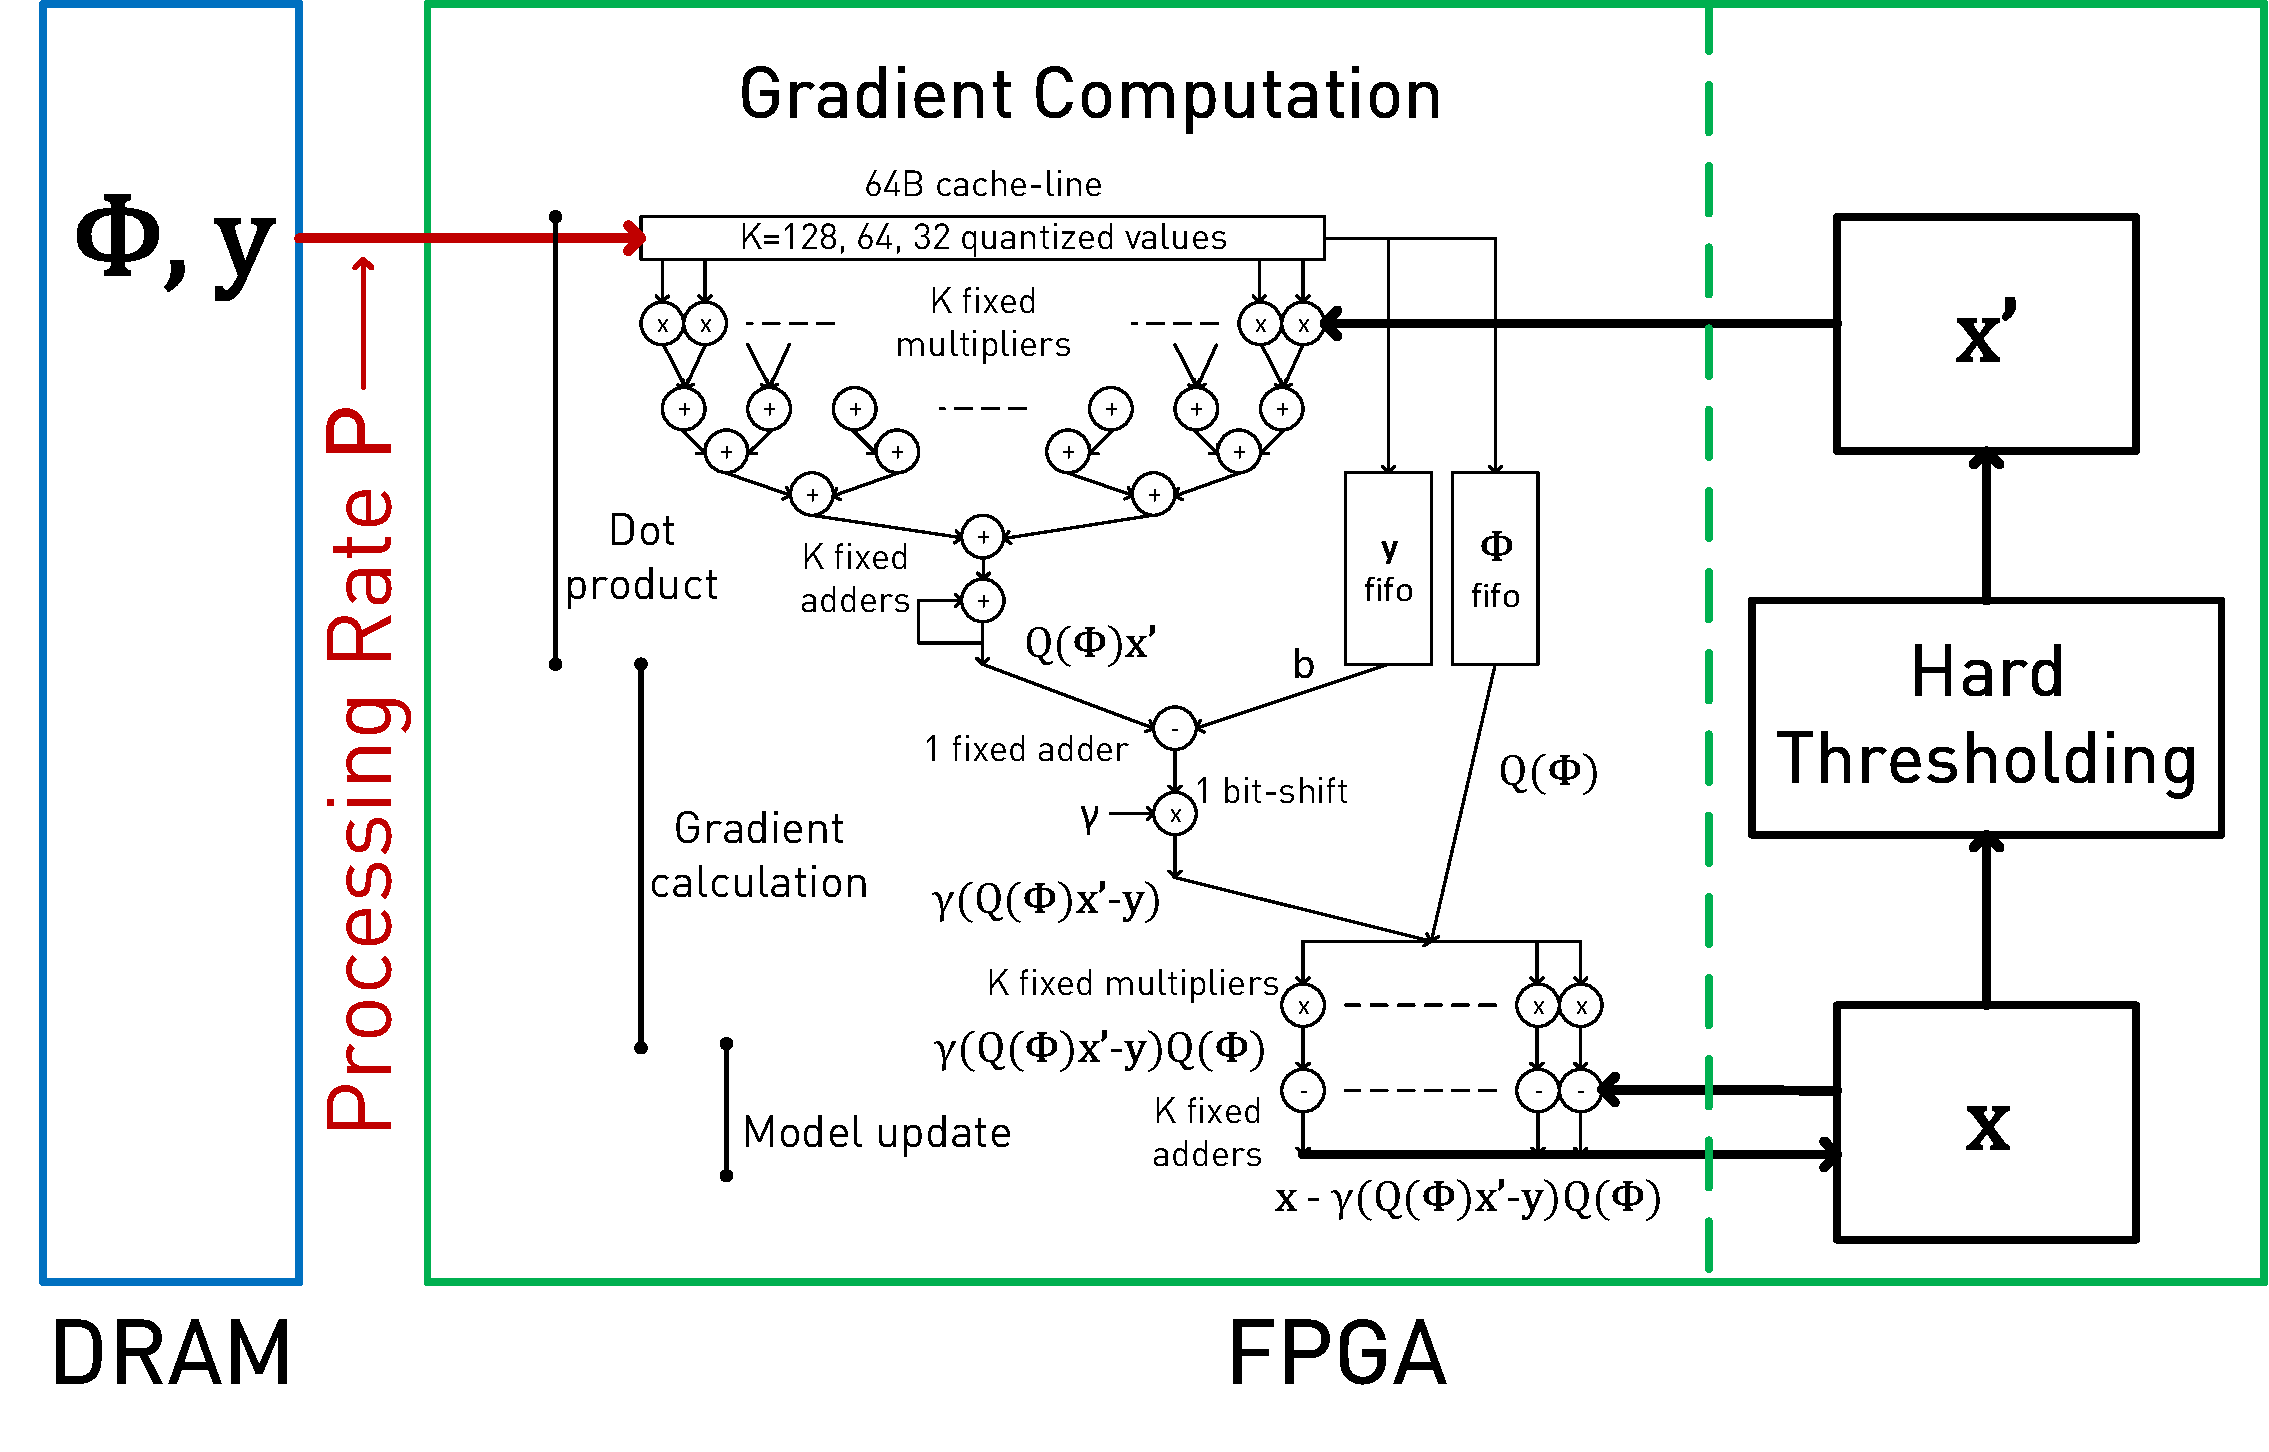
\includegraphics[width=0.5\columnwidth, angle=270]{figs/niht_fpga.eps}
\caption{NIHT on an FPGA-based system.}
\label{fig:fpga}
\end{figure}


{\bf Performance analysis:} The gradient computation unit as shown in Figure~\ref{fig:fpga} reads the measurement matrix ${\bf \Phi}$ and the measurements ${\bf y}$ from main memory and keeps {\bf x} in on-chip memory. It is able to process data from memory at ${\bf P}=12.8\,GB/s$. Thus, the design is bound on ${\bf P}$ for processing ${\bf \Phi}$ and ${\bf y}$. We achieve speed-up by quantizing ${\bf \Phi}$, because the time for each epoch is given by
$T = size({\bf \Phi})/{\bf P}$, since $size({\bf y}) \ll size({\bf \Phi})$. The essential trick for achieving linear speed-up is keeping ${\bf P}$ constant as the precision of ${\bf \Phi}$ is lowered (${\bf P}\to \land \, size({\bf \Phi})\downarrow$), which leads to more values arriving within each line from main memory. ${\bf P}$ can be kept constant on an FPGA, because we can adapt the gradient computation unit's microarchitecture and increase its internal parallelism to handle more values per incoming line. This is like having the ability to change the width of a vectorized instruction, which on a fixed microarchitecture as in a CPU or GPU is not possible.



\section{Experiments on a Real Telescope}
We assess the empirical performance of our algorithm solving imaging problem in radio astronomy on a real telescope: the LOw Frequency ARray (LOFAR) in Netherlands.
\subsection{Accuracy of Sky Recovery}
We image the full sky by employing 30 low-band antennas of LOFAR CS302 station that operates in 15-80 MHz frequency band where the sky is populated with 50 strong sources with signal-to-noise ratio of 0 dB at the antenna level, i.e., {\bf y}. 
\subsubsection{Improving the least square estimates}
Figure x provides an example of sky recoveries: (1) a least square estimate of underlying sky (or dirty image in the nomenclature of radio astronomy), (2) the ground truth estimated over 12 hours of observation, (3) 32-bits and (4) 2- bits iterative hard thresholding estimates using 10 seconds telescope data. This experiment indicates that low precision IHT captures the sky sources successively even when only 2-bits are used to compress its dense measurement matrix. This suggest that we can drastically reduce the observation time yet still estimate the sky precisely.



This empirical evidence is powerful yet not surprising. Mathematically, the measurement matrix we formed here hints on the distance between the antennas hence the phase relations. That is, each time a bit flips, we approximately know the change in x and y directions on the ground, which in turn permits us to form the phase relation at lower precision but still informative enough. 

%The reader might argue that, besides being on its most possible realistic setting, the above experiment does not fully capture the performance of low precision iht especially when only 2-bits are used to represent a dense measurement matrix. 

\subsubsection{Empirical comparison to the state-of-art methods}

We now present numerical comparisons of low precision IHT to the high precision IHT and other state-of-art methods, namely CoSaMP, CLEAN, $\ell_1$-based approach. The thread that binds all of these approaches in this experiment is their capability of good sparse support recovery. For this particular formulation of the interferometric imaging problem, they can iteratively build up an estimate of sky map ${\bf x}$. In order to avoid creating bias towards any algorithm, we implement these algorithms in a fair setting.

In radio interferometry, it is customary to use number of celestial sources resolved in the recovered image as a performance metric, i.e., true-positive findings. As such, we approach the evaluation of the algorithms here from two perspectives: (1) the exact sky recovery, (2) exact source recovery. That is, the performance of an algorithm is no longer described by its ability to recover support entirely but the sky objects, which possess higher error tolerance. This is illustrated in Figure. In fact, the current techniques are far beyond recovering the exact support precisely.

We demonstrate in Figure that IHT outperforms its alternatives in terms of its source resolution capability even at the low precision setting and at various SNR levels. The empirical results suggest that the celestial sources can still be recovered by dramatically compressing the measurement matrix.

Recall from the former discussions that noise in receivers is far stronger than the weak incoming signals thus low SNR at the antenna level results, i.e., usually ranged from -5 to 5 dB. The robustness of those alternative approaches to the noise is also depicted in Figure. Clearly, the CLEAN algorithm notably underperforms in the presence of significant noise. This undesirable property is yet not surprising. A careful look into the the algorithmic steps, it apparently matches also to the noise artefacts in the image considering them as a point source. The performance of IHT and CoSaMP remain good, illustrates by Figure x.


{\it Discussions on these results:} This experiment is informative merely on the accuracy of the results obtained implementing these alternative algorithms. A fair comparison involves the analysis of different properties such as speed and storage requirements, flexibility and ease of implementation. Capsulizing briefly, CoSaMP has strong theoretical guarantee when the least squares solution is supplied and requires the solution to an inverse problem at each iteration, which is costly in general and demands better storage capability niht8. On the other hand, IHT is shown to outperform CoSaMP and have significant speed advantage refbooks. The empirical evidence further suggest that IHT performs nearly as well as the $\ell_1$-based approach. Finally, the CLEAN requires a 2D Fourier inversion and deconvolution per iteration thus the operational expense of the method is relatively higher compared to those of IHT and CoSaMP -13tez. Sharing similar performance guarantees with the high precision IHT, low precision approach thus seems powerful considering all these aspects. This is evident in Figure.

In real-life problems usually lack of traditional restricted isometry property. The scale-invariant feature of the measurement matrix used in normalized IHT however alleviates the RIP condition and imposes a fairly mild constraint in ref-eqn. The choice of the algorithm is thus desired to satisfy refeq with high probability. In a series of paper refs, CoSaMP is shown to perform markedly worse when the RIP condition fails. IHT, however, still preserves its near-optimal recoveries far beyond the region of RIP. While this favors IHT over CoSaMP, there is no rigid assumption imposed on the CLEAN and $\ell_1$-based approach. 
 


% \., which is vastly superior to the resitual in...
% This suggest we can drastically reduce bidi bidi
% Such a result has potentially profound consequences for the power consumption.


\subsubsection{Monitoring RIP and recovery error}
Using the strategy introduced in [], we monitor the restricted isometry constants $\gamma_{2s}$ and $\hat{\gamma}_{2s}$ and the recovery error in order to investigate (1) if the RIP condition is more sensitive, (2) how the condition and recovery performance are related to each other, in the low precision setting compared to the high precision IHT.

Figure. demonstrates that ...






\subsection{Speed-up on FPGA}





\section{Discussion}







\newpage
\cite{iht}
\cite{niht}
\cite{greedy_algorithms}
% In the unusual situation where you want a paper to appear in the
% references without citing it in the main text, use \nocite
\nocite{langley00}

\bibliography{references}
\bibliographystyle{icml2018}


\end{document} 

